\documentclass{article}

%in that file you will find the packages and other macro needed like \R for the
%real number set.
\usepackage{vmargin}
\setmarginsrb{28mm}{25mm}{28mm}{25mm}{0pt}{0mm}{0pt}{0mm}
\setlength{\footskip}{20pt}
\usepackage{amssymb}
\usepackage{amsmath}
\usepackage{amsthm}
\usepackage{pgfplots}
\pgfplotsset{compat=1.9} % for backward compatibility
\usepackage{graphicx}
\usepackage[utf8]{inputenc}
\usepackage{tikz}
\usepackage{bbm}
\usepackage{subcaption}
% \usepackage[boxruled]{algorithm2e}
\usepackage{algpseudocode}
\usepackage{algorithm}
\usetikzlibrary{positioning}
\usepackage{caption}
\usepackage{mathtools}
\usepackage{lipsum}
\usepackage[title,titletoc]{appendix}
\usepackage{booktabs}
\usepackage{here}
%Literatur
\usepackage[%
    backend=biber,
    sortcites, % sort automatically
    sorting=nty, % sort order
    safeinputenc, % solves problems with unicode-formatted author names etc.
    citestyle=alphabetic, %
    bibstyle=alphabetic, %
    hyperref=true, % provide clickable links
    maxbibnames=3, % shorten author list for more than 3 names
    maxcitenames=3, % use at most 3 names for key
    url=false, % do not print URLs
    doi=false, % do not print DOIs
    giveninits=true,
    ]%
{biblatex}
% automatische Anführungszeichen
\usepackage[autostyle=true]{csquotes}
\usepackage[hidelinks]{hyperref}
%some weird packages
\usepackage{halloweenmath}
\usepackage{txfonts}
\usepackage{knitting}
\usepackage{listings}
\usepackage{xcolor}
\usepackage{multirow}
\usepackage{wrapfig}

\definecolor{codegreen}{rgb}{0,0.4,0}
\definecolor{codegray}{rgb}{0.5,0.5,0.5}
\definecolor{mymauve}{rgb}{0.58,0,0.82}
\definecolor{codepurple}{rgb}{0.58,0,0.82}
\definecolor{backcolour}{rgb}{0.95,0.95,0.92}

\lstdefinestyle{mystyle}{
    %backgroundcolor=\color{backcolour},
    commentstyle=\color{codegreen},
    keywordstyle=\color{mymauve},
    numberstyle=\tiny\color{codegray},
    stringstyle=\color{codepurple},
    basicstyle=\ttfamily\footnotesize,
    breakatwhitespace=false,
    breaklines=true,
    captionpos=b,
    keepspaces=true,
    numbers=left,
    numbersep=5pt,
    showspaces=false,
    showstringspaces=false,
    showtabs=false,
    tabsize=2
}

\lstset{style=mystyle}

\DeclarePairedDelimiter{\ceil}{\lceil}{\rceil}
\renewcommand{\phi}{\varphi}
\newcommand{\eqtext}[1]{\ensuremath{\stackrel{#1}{=}}}
\newcommand{\leqtext}[1]{\ensuremath{\stackrel{#1}{\leq}}}
\newtheorem{theorem}{Proposition}[section]
\newtheorem{lemma}{Lemma}[section]
\newtheorem{remark}{Remark}[section]
\newcommand{\N}{\mathbb{N}}
\newcommand{\R}{\mathbb{R}}
\newcommand{\E}{\mathbb{E}}
\newcommand{\epl}{\varepsilon}

\renewcommand{\algorithmicrequire}{\textbf{Input:}}
\renewcommand{\algorithmicensure}{\textbf{Output:}}

\theoremstyle{definition}
\newtheorem{definition}{Definition}[section]

\addbibresource{Project2.bib}

\date{\today}

\begin{document}

%this creates the title page. You must complete the information there
\hypersetup{pageanchor=false}
\begin{titlepage}
\newcommand{\HRule}{\rule{\linewidth}{0.5mm}} % Defines a new command for the horizontal lines, change thickness here

\center % Center everything on the page

%----------------------------------------------------------------------------------------
%   HEADING SECTIONS
%----------------------------------------------------------------------------------------

\vspace{3cm}
\textsc{\LARGE École polytechnique fédérale de Lausanne}\\[1.5cm] % Name of your university/college
\textsc{\Large HPC for Numerical Methods and Data Analysis}\\[0.5cm] % Major heading such as course name
\textsc{\large Course Project Fall 2023}\\[0.5cm] % Minor heading such as course title

%----------------------------------------------------------------------------------------
%   TITLE SECTION
%----------------------------------------------------------------------------------------

\HRule \\[0.4cm] % line above and under the title
{ \huge \bfseries Randomized Nyström Low-Rank Approximation}\\[0.4cm] % Title of your document
\HRule \\[1.5cm]

%----------------------------------------------------------------------------------------
%   AUTHOR SECTION
%----------------------------------------------------------------------------------------

\begin{minipage}{0.4\textwidth}
\begin{flushleft} \large
\emph{Authors:}\\
Christian \textsc{Mikkelstrup}\\
Julian Philipp \textsc{Schmitt} % Your name
\end{flushleft}
\end{minipage}
~
\begin{minipage}{0.4\textwidth}
\begin{flushright} \large
\emph{Supervisor:} \\
Prof. Laura \textsc{Grigori} % Supervisor's Name
\end{flushright}
\end{minipage}\\[10cm]

%----------------------------------------------------------------------------------------
%   LOGO SECTION
%----------------------------------------------------------------------------------------


\includegraphics[width=0.4\linewidth]{Logo}\\[1cm] % Include a department/university logo - this will require the graphicx package

%----------------------------------------------------------------------------------------

\vfill % Fill the rest of the page with whitespace

\end{titlepage}


\clearpage
\thispagestyle{empty}
\tableofcontents

\clearpage
\hypersetup{pageanchor=true} % to start numbering after title and ToC pages
\pagenumbering{arabic}
\setcounter{page}{1}

\section{Introduction}
In this project, we study the randomized Nyström approximation algorithm for the low-rank approximation of a positive-semidefinite matrix $A\in \mathbb{R}^{n \times n}$. There are several important applications for this theory, such as image processing, PCA or solving integral equations. However, the most common practical setting are kernel methods for large-scale machine learning problems. Since these algorithms scale at least quadratic in the number of data points, low-rank approximations are essential to obtain reasonable storage usage and computational costs. 

The randomized Nyström approximation is based on a sketching matrix $\Omega \in \mathbb{R}^{n \times l}$ and the formula:
\begin{align}
    \label{nyst:sketching_formula}
    A_{Nyst} = (A \Omega) (\Omega^T A \Omega)^+ (\Omega^T A)
\end{align}
where $l \ll n$ is the sketching dimension and $(\Omega^T A \Omega)^+$ denotes the pseudo-inverse. In particular, our algorithm will compute a fixed-rank $k \leq l$ approximation by truncating the sketched matrix $A_{Nyst}$. Key aspects of our research are numerical stability, scalability, performance and the approximation of the leading $k$ singular values of $A$.

We used \cite{golub2013a}.
*** clearly missing something...???***

\section{Randomized Nyström Algorithm}\label{sec:rand_nystrom_alg}
In this section, we describe the efficient computation of a rank-k approximation from the sketching formula (\ref{nyst:sketching_formula}). We obtain such an approximation by simply truncating the \textit{singular value decomposition} (SVD) of $A_{Nyst}$. In literature, this method is also called \textit{modified fixed-rank Nyström via $QR$}. However, instead of calculating the entire SVD of $A_{Nyst}$ and throwing away the rows and columns we do not need, if $k<l$, we compute the partial SVD, extracting only the $k$ singular values of the largest magnitude \cite{scipy_svds}. Algorithm \ref{algo:nyström} shows a way for computing $[A_{Nyst}]_k$. The algebra behind the algorithm is the following: Let $C = A \Omega$ and $B = \Omega^T A \Omega$. Furthermore, we write $B = LL^T$ for the Cholesky decomposition of $B$, $Z = C L^{-T} = QR$ for the $QR$ decomposition of $C L^{-T}$ and $R = U_k \Sigma_k V_k^T$ for the truncated SVD of $R$. Now, we obtain
\begin{align*}
    A_{Nyst} = (A \Omega) (\Omega^T A \Omega)^+ (\Omega^T A) &= CL^{-T}L^{-1}C^T = ZZ^T \\
    &= QRR^TQ^T = QU_k\Sigma_k \Sigma_k^T U_k^TQ^T = QU_k\Sigma_k^2 U_k^TQ^T.
\end{align*}
 Note that in step 7 of Algorithm \ref{algo:nyström}, instead of computing $\hat{U}_k$ as $Q U_k$ we could use $\hat{U}_k = Z V_k \Sigma_k^{-1}$, which would provide less numerical stability but entail a smaller computational cost. In particular, one could omit the computation of the $Q$-factor of the $QR$ decomposition. Moreover, it is important to mention that the matrix $B = \Omega^T A \Omega$ can be rank-deficient, e.g. if the rank of $A$ or $\Omega$ is smaller than $l$. In this case, it is not possible to obtain the Cholesky factorization in step 3. Instead, one can use the square root of an SVD or the eigendecomposition of $\Omega^T A \Omega$. Finally, we remark that Algorithm \ref{algo:nyström} is a is a \textit{streaming} algorithm since it requires only one pass over the data or $A$, respectively. This is a major advantage compared to e.g. the randomized singular value decomposition.
\begin{algorithm}[H]
    \caption{Randomized Nyström} \label{algo:nyström}
    \begin{algorithmic}[1]
        \Require $A \in \mathbb{R}^{n \times n}, \Omega \in \mathbb{R}^{n \times l}$
        \State $C = A \Omega \in \mathbb{R}^{n \times l}$
        \State $B = \Omega^T C \in \mathbb{R}^{l \times l}$
        \State $B = LL^T$ (via Cholesky)
        \State $Z = C L^{-T}$ (via substitution on triangular system)
        \State $Z = QR$ ($QR$ decomposition)
        \State Compute rank-k SVD of $R$: $U_k \Sigma_k V_k^T$
        \State $\hat{U}_k = Q U_k$
        \Ensure $[A_{Nyst}]_k = \hat{U}_k \Sigma^2 \hat{U}_k^T$
    \end{algorithmic}
\end{algorithm}

\subsection{Sketching Techniques}
In this section, we describe the construction of the sketching matrix $\Omega \in \mathbb{R}^{n \times l}$. In particular, we are concerned with randomized methods for dimension reduction and it is therefore useful to define the so-called \textit{oblivious $l_2$-subspace embedding} (OSE):
\begin{definition}[OSE]
    Let $0 < \epsilon < 1$ and $0 < \delta < 1$. A random matrix $\Omega \in \mathbb{R}^{n \times l}$ is a $(\epsilon, \delta, d)$ OSE, if for any fixed $d$-dimensional subspace $V \subseteq \mathbb{R}^{n}$, 
    \begin{align*}
        \left| ||x||_2^2 - ||\Omega^T x||_2^2 \right| \leq \epsilon \cdot ||x||_2^2
        \quad \forall x \in V 
    \end{align*}
    holds with probability $1 - \delta$.
\end{definition}

For the randomized Nyström approximation, we considered two different sketching techniques: the \textit{block Subsampled Randomized Hadamard Transform} (BSRHT) and a \textit{Short-Axis-Sparse Sketching Operator} (SASO). Both are sparse and structured random matrices which aim to reduce the computational costs of the matrix-matrix product $A \Omega$.

The BSRHT is a version of the Subsampled Randomized Hadamard Transform (SRHT) specifically designed for distributed architectures. For $n$ being a power of two, the SRHT can be defined as
\begin{align*}
    \Omega^T = \sqrt{\frac{n}{l}} R H D
\end{align*}
where
\begin{itemize}
    \item $H\in \mathbb{R}^{n \times n}$ is the normalized Walsh–Hadamard matrix which is defined recursively as:
    \begin{align*}
        H_2 = \begin{pmatrix}
            1 & 1 \\
            1 & -1
        \end{pmatrix}, 
        \qquad
        H_n = \begin{pmatrix}
            H_{n/2} & H_{n/2}\\
            H_{n/2} & -H_{n/2}
        \end{pmatrix}
        \qquad \text{and} \qquad
        H = n^{-1/2} H_n
    \end{align*}
    \item $D\in \mathbb{R}^{n \times n}$ is a diagonal matrix with i.i.d. RVs $\sim$ Uniform$(\{\pm 1\})$
    \item $R\in \mathbb{R}^{n \times l}$ is a subset of $l$ randomly sampled rows from the $n \times n$ identity matrix
\end{itemize}
Now, for $P$ different processors, the BSRHT can be constructed block-wise from the SRHT as:
\begin{align}
    \label{BRSHT}
    \Omega^T
    = \begin{pmatrix}
        \Omega_1 & \ldots & \Omega_P 
    \end{pmatrix} 
    = \sqrt{\frac{n}{Pl}} 
    \begin{pmatrix}
        D_{L1} & \ldots & D_{LP} 
    \end{pmatrix} 
    \begin{pmatrix}
        RH \\
        & \ddots \\
        && RH
    \end{pmatrix}
    \begin{pmatrix}
        D_{R1}\\
        & \ddots \\
        && D_{RP}
    \end{pmatrix}
\end{align}
with 
\begin{itemize}
    \item $H\in \mathbb{R}^{n/P \times n/P}$ being the normalized Walsh–Hadamard matrix.
    \item $D_{L i}\in \mathbb{R}^{l \times l}, D_{R i}\in \mathbb{R}^{n/P \times n/P}$ being diagonal matrices with i.i.d. Rademacher entries $\pm 1$
    \item $R\in \mathbb{R}^{l \times n/P}$ being a  uniform sampling matrix
\end{itemize}
The main advantage of the BRSHT compared to the SRHT is that the matrix-matrix product distributed across $P$ processors with row-wise partitioning can be computed as $A\Omega = \sum_{i=1}^P A_i \Omega_i$. In particular, one can compute the local contributions $A_i \Omega_i$ independently on each processor and finally sum-reduce them. Note that since exactly the same $R$ has to be generated on each processor, the root processor has to broadcast a seed for generating this sampling matrix. \citeauthor{balabanov2022} \cite{balabanov2022} showed that the construction of $\Omega$ as in (\ref{BRSHT}) yields an $(\epsilon, \delta, d)$ \textit{oblivious subspace embedding} (OSE) if
\begin{align}
    \label{BRSHT:OSE_Condition}
    n \geq l \geq 3.7 \epsilon^{-2} 
    \left( 
        \sqrt{d} + 4 \sqrt{\log \frac{n}{\delta} + 6.3}
    \right)^2
    \log \frac{5d}{\delta}
\end{align}
with $0 < \epsilon < 1$ and $0 < \delta < 1$. This implies compatability with all randomized methods that rely on OSEs and in particular with the Nyström approximation. Note that condition (\ref{BRSHT:OSE_Condition}) can be used to choose a proper sketching dimension $l$.

For the construction of the SASO, we call the rows of $\Omega$ \textit{short-axis vectors} since $l \ll n$. These short-axis vectors should be independent of one another and have a small, fixed number of non-zero elements. In general, there are different ways of selecting the locations of the non-zero elements. We decided to sample $k$ indices uniformly from $[l]$ without replacement, once for each row. Furthermore, the values of the non-zeros are drawn independently and uniformly from $[-2,-1] \cup [1, 2]$. Compared to i.i.d. Rademachers this can protect against the possibility of a given column of $\Omega$ being orthogonal to a row of $A$ \cite{murray2023}. Finally, we set $k = \min\{8, l\}$ following experimental results metioned in \cite{murray2023}.

\section{Parallelization of the Nyström Algorithm}\label{sec:parallel_nystrom}
Having seen the (sequential) randomized Nyström approximation in Algorithm \ref{algo:nyström}, we focus now on the corresponding parallelization for a distributed system. For $A \in \mathbb{R}^{n \times n}$ and $\Omega \in \mathbb{R}^{n \times l}$, the Nyström approximation can be divided into 4 steps:
\begin{enumerate}
    \item Sketching: $C = A \Omega \in \mathbb{R}^{n \times l}, B = \Omega^T C \in \mathbb{R}^{l \times l}$
    \item Decomposition: $B = LL^T$ (e.g. via Cholesky) with $L \in \mathbb{R}^{l \times l}$ and $Z = C L^{-T} \in \mathbb{R}^{n \times l}$
    \item $QR$ factorization: $Z = QR$ with $Q \in \mathbb{R}^{n \times l}$ and $R \in \mathbb{R}^{l \times l}$
    \item Rank-k SVD of $R$: $U_k \Sigma_k V_k^T$ and $\hat{U}_k = Q U_k$
\end{enumerate}
Considering $l \ll n$, we aim to parallelize the sketching of $A$ and use the TSQR algorithm for the $QR$ factorization of the tall-skinny matrix $Z$. The decomposition of $B$ and the SVD of $R$ can be computed sequentially since both matrices are small.

For the parallel sketching, we work with a 2D block distribution of $A$ and a row-block distribution of $\Omega$. From now on, we assume w.l.o.g. that the number of processors $P$ is a power of 4 because we need $\sqrt{P}$ to be an integer for the 2D distribution and later we will need a power of 2 for TSQR. Note that this can always be achieved by zero padding of the input data. For $P=4$, the matrix partitioning is the following:
\begin{align*}
    C = A \Omega 
    = \begin{pmatrix}
        A_{11} & A_{12} \\
        A_{21} & A_{22}
    \end{pmatrix}
    \begin{pmatrix}
        \Omega_1 \\
        \Omega_2
    \end{pmatrix}
    &= \begin{pmatrix}
        A_{11} \Omega_1 + A_{12} \Omega_2 \\
        A_{21} \Omega_1 + A_{22} \Omega_2
    \end{pmatrix}
    \\
    B = \Omega^T C
    = \begin{pmatrix}
        \Omega_1^T & \Omega_2^T
    \end{pmatrix}
    \begin{pmatrix}
        C_1 \\
        C_2
    \end{pmatrix}
    &= \begin{pmatrix}
        \Omega_1^T & \Omega_2^T
    \end{pmatrix}
    \begin{pmatrix}
        A_{11} \Omega_1 + A_{12} \Omega_2 \\
        A_{21} \Omega_1 + A_{22} \Omega_2
    \end{pmatrix}
\end{align*}
The sketching algorithm works by first computing $C$ and then using $C$ to compute $B$. Algorithm \ref{algo:sketching} illustrates the procedure. For each processor owning a block $A_{ij} \in \mathbb{R}^{n/\sqrt{P} \times n/\sqrt{P}}$, we start by generating the corresponding block $\Omega_j \in \mathbb{R}^{n/\sqrt{P} \times l}$ of the sketching matrix. Then, we compute $C_{ij} = A_{ij} \Omega_j$ in parallel and sum reduce among processors in the same row $C_i = \sum_{j = 1}^{\sqrt{P}} C_{ij}$. For the computation of $B$, we need to sketch each $C_i$ from the left by multiplying $\Omega_i$. Note that for processors owning a diagonal block $A_{ii}$, it holds $\Omega_i = \Omega_j$ and we do not have to generate $\Omega_i$. Therefore, we choose the processors owning a diagonal block $A_{ii}$ of $A$ as roots for the reduce operation. Now, we could simply compute $\Omega_i^T C_i$ on the $\sqrt{P}$ processors owning a $C_i$ block and then sum reduce among these to obtain $B$. However, later we want to execute the TSQR algorithm on all $P$ processors using a row-block distribution of $C$. Therefore, we chose to scatter $C$ already during sketching and exploit the additional processing power for the computation of $B$. We scatter each $C_i$ among processors in the same column because these processors do all own the same sketching matrix $\Omega_i$. Since we partitioned $C_i \in \mathbb{R}^{n/\sqrt{P} \times l}$ into $C_{ij} \in \mathbb{R}^{n/P \times l}$, each processor uses only a row-block of $\Omega_i$ for sketching and has to compute $B_{ij} = \Omega_i[i \cdot n/P : (i+1) n/P, :]^T C_{ij}$. Finally, we sum-reduce $B = \sum_{i,j = 1}^{\sqrt{P}, \sqrt{P}} B_{ij}$ among all processors. Note that the matrix $C$ is row-block distributed and $B$ is owned exclusively by the root processor after sketching.

Next, the decomposition of $B= LL^T$ is computed sequentially only on the root processor. The matrix $L$ is then broadcasted to compute $Z = C L^{-T}$ in parallel. The algebra for 4 processors is:
\begin{align*}
    Z = C L^{-T} 
    = \begin{pmatrix}
        C_1 \\
        C_2 \\
        C_3 \\
        C_4
    \end{pmatrix}
    L^{-T} 
    = \begin{pmatrix}
        C_1 L^{-T} \\
        C_2 L^{-T} \\
        C_3 L^{-T} \\
        C_4 L^{-T}
    \end{pmatrix}
\end{align*}
(Of course, we do not work with the inverse matrix $L^{-T}$, but compute $Z$ via a linear system.) The advantage of the parallelized approach is that we do not need to gather $C$ together and can compute $Z$ directly distributed row-block wise which we need anyway for the TSQR algorithm in the next step.

In the third step, we compute the $QR$ factorization of the tall and skinny matrix $Z$. We use the (parallel) TSQR algorithm which uses a reduction-like operation among a binary tree of processors to compute $Q$ and $R$ in parallel. It is communication optimal and as stable as Householder $QR$. For details, we refer to \cite{demmel2008}. At the end, the $Q$ factor is returned distributed row-block wise while $R$ is owned by the root processor.

In the final step, we copute the rank-k truncated SVD $U_k \Sigma_k V_k^T$ of $R$ and $\Sigma_k^2$ sequentially on the root processor. Then, we broadcast $U_k$ to compute $\hat{U}_k = Q U_k$ in parallel ($Q$ is still row-block distributed) and gather $\hat{U}_k$ together. We return $\Sigma_k^2$ as well as $\hat{U}_k$ on the root processor.

\begin{algorithm}[t]
    \caption{Parallel Sketching} \label{algo:sketching}
    \begin{algorithmic}[1]
        \Require $A \in \mathbb{R}^{n \times n}, \Omega \in \mathbb{R}^{n \times l}$
        \State Root processor: broadcast information for generating blocks of Ω
        \For{\text{all processors $P_{ij}$ with $i,j = 1:\sqrt{P}$ in parallel}}
            \State Generate block $\Omega_j$
            \State Compute $C_{ij} = A_{ij} \Omega_j$
            \State Sum-Reduce among rows $C_i = \sum_{j = 1}^{\sqrt{P}} C_{ij}$ with root being $P_{ii}$
            \State Scatter $C_i$ among processors in same column
            \State Compute $B_{ij} = \Omega_j[i \cdot n/P : (i+1) n/P, :]^T \ C_{ij}$
        \EndFor
        \State Sum-Reduce $B = \sum_{i,j = 1}^{\sqrt{P}, \sqrt{P}} B_{ij}$
        \Ensure $B, C$
    \end{algorithmic}
\end{algorithm}

\section{Datasets}\label{sec:datasets}

In the following sections, we will investigate the performance of the Nyström algorithm on 5 different datasets. The positive semi-definite matrices will be made from both real and synthetic data, as described in this section. For all datasets we chose to subsample the datapoints for the real data, or simply choose the dimension for the synthetic data such that we had $n=8.192$, leading to a positive semi-definite matrix $A\in\mathbb{R}^{n\times n}$. In all experiments, all datasets were run with the different sketching matrices ($\Omega$), sketching dimensions (l), and approximation ranks (k). We had a total of 19 different $(l,k)$ pairs with $l$ ranging from $400$ to $2000$ and $k$ ranging from $100$ to $900$. Note that this choice of parameters is specific to us using $P=4$ processors with TSQR. This enables us to use the \textit{tall and skinny} QR factorization on $Z\in\mathbb{R}^{n\times l}$ for all our parameters since $n\geq 4\cdot l$.\newline

For the matrices created from real data, we used the MNIST and YearPredictionMSD datasets \cite{726791, Bertin-Mahieux2011}. We then used a subset of $n=8.192$ datapoints, and used the radial basis function (RBF), $A_{i,j}=e^{-||x_i-x_j||_2^2}/{\sigma^2}$ to create a symmetric and positive semi-definite matrix. For MNIST, we chose a value of $\sigma=100$, and for YearPredictionMSD we chose $\sigma=10^4$ and $\sigma=10^5$ for a total of three datasets, matching the approach in \cite{balabanov2022}. \newline
For the synthetic datasets, we choose diagonal matrices containing positive elements with different rates of decay for the singular values. Since $A$ is a diagonal matrix, we can easily select the singular values, and thus also choose an effective rank, $R$, of the matrices. We used both a \textit{Polynomial decay} and an \textit{Exponential decay} of the singular values. The matrix with \textit{Polynomial decay} has the form
\begin{equation*}
A=\text{diag}(\underbrace{1,...,1}_R,2^{-p}, 3^{-p}, ..., (n-R+1)^{-p})\in\mathbb{R}^{n\times n}.
\end{equation*}
The parameter $p>0$ is a hyperparameter used to control the decay of the polynomially decaying singular values. The matrix with \textit{Exponential decay} has the form
\begin{equation*}
A=\text{diag}(\underbrace{1,...,1}_R,10^{-q}, 10^{-2q}, ..., 10^{-(n-R)q})\in\mathbb{R}^{n\times n}
\end{equation*}
The parameter $q>0$ again controls the rate of decay, now of the exponentially decaying singular values. To match the datasets in \cite{tropp2017fixedrank}, we set $R=10$, $p=1$, and $q=0.25$ for all experiments, also matching the real datasets in size by setting $n=8.192$, leading to two synthetic datasets.

\section{Numerical Stability} \label{sec:num_stability}
%  An investigation of the numerical stability of randomized Nystr¨om. For the data sets described in section 2.1, you should provide graphs that display the error of the low rank approximation in terms of nuclear norm (norm(A, 'nuc')). The error to be studied experimentally is kA−[[ANyst]]kk∗/kAk∗. The discussion should compare as well the accuracy obtained for the two different sketching matrices by taking into consideration the sketching dimension. This investigation should be done on the data sets provided in 2.1. Additional data could be provided but is not required.

The numerical performance is tested on the datasets described in \ref{sec:datasets}. The performance is measured using the relative error with the nuclear norm,
\begin{equation}
    \textit{Relative error is: } \frac{||A-\llbracket A_{nyst}\rrbracket_k||_*}{||A||_*}.
\end{equation}
Since the nuclear norm is the sum of the singular values, $||A||_*=\sigma_1(A)+...+\sigma_n(A)$, this value describes the ratio of the sum of the singular values from the approximation error of $\llbracket A_{nyst}\rrbracket_k$, compared to the original matrix $A$. If this value is low, we have a good low-rank approximation of $A$. \newline

We used the parallel randomized Nyström with Cholesky for all datasets except for the exponential synthetic dataset. For this dataset, Cholesky failed with the error message that $B$ was a singular matrix. For this dataset, we instead used ***the svd version(what is name of this)***. Because of the performance differences, as seen in section \ref{sec:performance}, we chose to use the svd version only for this dataset.\newline

The relative error for all datasets and both sketching matrices can be seen in figure \ref{fig:RelError}. For all the tests except the exponential decay dataset, we could see a monotonic reduction in relative error using a larger size of $l$ or $k$, if the other value was kept fixed. However, when keeping $l$ fixed, even though the relative error was reduced when increasing $k$, we found a reduction in the improvement for each step. That is, we get diminishing returns on the improvement in the relative error when increasing the approximation rank, $k$. The exception to this is the exponential dataset. Changing the approximation rank makes the numerical performance jump both up and down. We even see that for the BSRHT sketching matrix, increasing the sketching dimension has a slightly worse relative error. However, for all tests run with the exponential dataset, the relative error was less than $10^{-14}$, which is close to the machine precision, and significantly lower than all other considered datasets. \newline

Comparing across the different datasets, we see a big difference in the magnitude of the relative errors. The polynomial dataset has a much larger relative error, compared to all other datasets, and the YearPredictionMSD dataset with $\sigma=10^5$ is significantly better than all other datasets (except the exponential decay mentioned before), across all combinations of different hyperparameters. This also shows that for the YearPredictionMSD dataset, the value for $\sigma$ has a much larger impact on the relative error than the values for the sketching dimension or the approximation rank. It seems that datasets created with a smaller standard deviation in the radial basis function, are easier to approximate using the randomized Nyström approximation. (***After creating the singular value plots, maybe compare year1e-5 to exp???*** Maybe just bridge to singular value plots???***). \newline

Another interesting finding across datasets is that when fixing a low approximation error, the difference in relative error when varying the sketching dimension, depended heavily on the initial performance. That is, if we found a low relative error for a low approximation rank, increasing the sketch dimension made little to no difference, but when the initial performance was poor, as with the dataset with polynomial decay, we did see some difference. So if one were to select between increasing the sketch dimension or the approximation rank to get the most improvement in the relative error, the results were not conclusive. However, as a general trend, for a low approximation rank, we found the most improvement by increasing the approximation rank, and for medium to high approximation ranks we found more significant improvements by increasing the sketch dimension.\newline

Comparing across different sketching matrices, we find next to identical results. That is, in our testing, we did not find any significant numerical differences between the two different sketching matrices. The only visible difference across sketching matrices was for the exponential decay dataset. Here we found that the BSRHT sketching matrix, had a systematic worse approximation error when increasing the sketching dimension, though still close to machine precision. This increasing behavior was not observed with the SASO sketching matrix, closer matching what we found for the other datasets, which in turn also had a lower relative error. 

% Relative error plots - describe what we see/have found

\begin{figure}
\centering
\hfill\begin{subfigure}[t]{\dimexpr0.4\textwidth+20pt\relax}
    \makebox[20pt]{\raisebox{65pt}{\rotatebox[origin=c]{90}{MNIST}}}%
    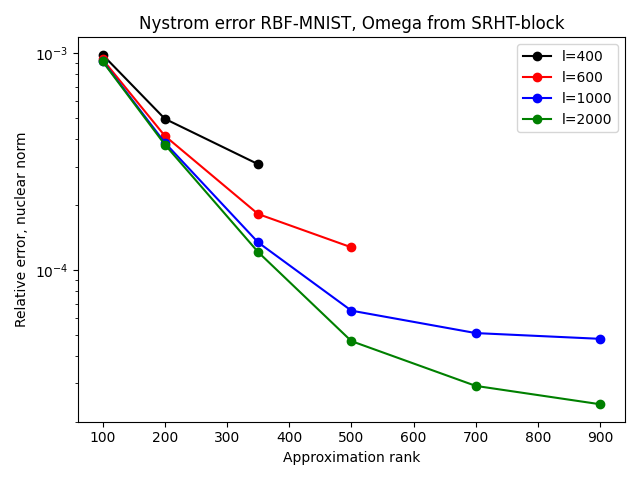
\includegraphics[width=\dimexpr\linewidth-20pt\relax]{plots/relerror/relerror_RBF-MNIST_SRHT-block.png}
    \makebox[20pt]{\raisebox{65pt}{\rotatebox[origin=c]{90}{YearMSD, $\sigma=10^4$}}}%
    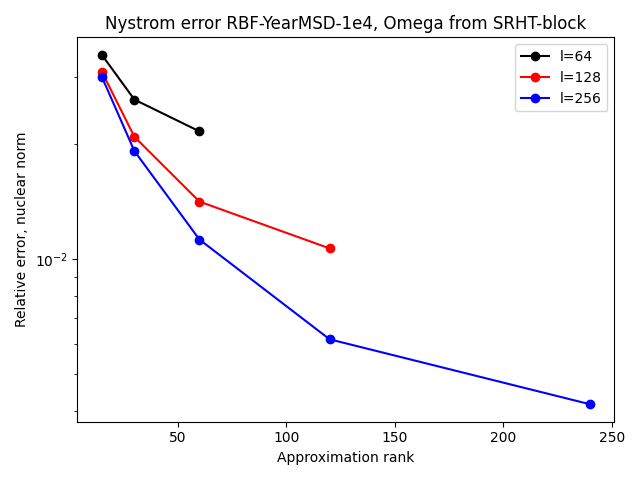
\includegraphics[width=\dimexpr\linewidth-20pt\relax]{plots/relerror/relerror_RBF-YearMSD-1e4_SRHT-block.png}
    \makebox[20pt]{\raisebox{65pt}{\rotatebox[origin=c]{90}{YearMSD, $\sigma=10^5$}}}%
    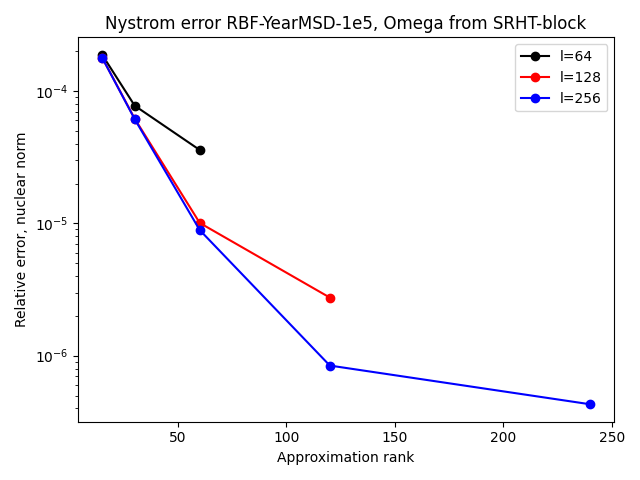
\includegraphics[width=\dimexpr\linewidth-20pt\relax]{plots/relerror/relerror_RBF-YearMSD-1e5_SRHT-block.png}
    \makebox[20pt]{\raisebox{65pt}{\rotatebox[origin=c]{90}{Polynomial decay}}}%
    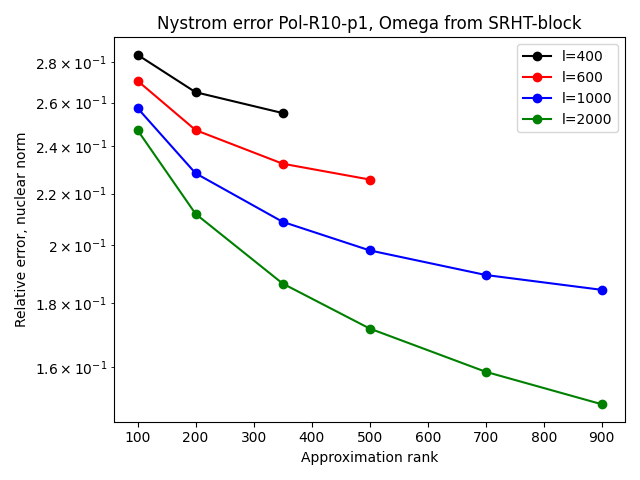
\includegraphics[width=\dimexpr\linewidth-20pt\relax]{plots/relerror/relerror_Pol-R10-p1_SRHT-block.png}
    \makebox[20pt]{\raisebox{65pt}{\rotatebox[origin=c]{90}{Exponential decay}}}%
    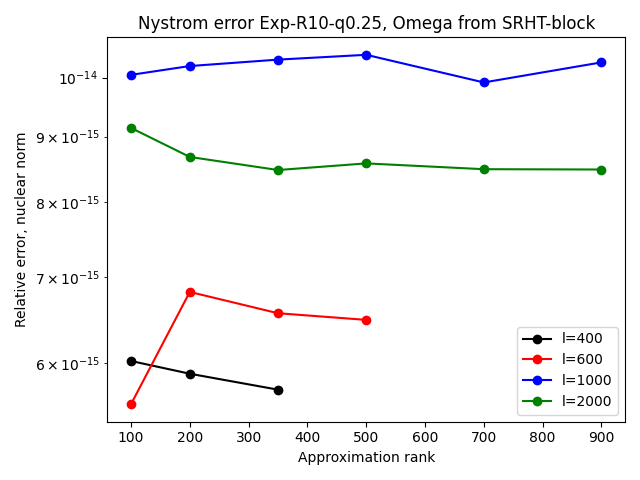
\includegraphics[width=\dimexpr\linewidth-20pt\relax]{plots/relerror/relerror_Exp-R10-q0.25_SRHT-block.png}
    \caption{$\Omega$ created using BSRHT}
\end{subfigure}\hfill
\begin{subfigure}[t]{0.4\textwidth}
    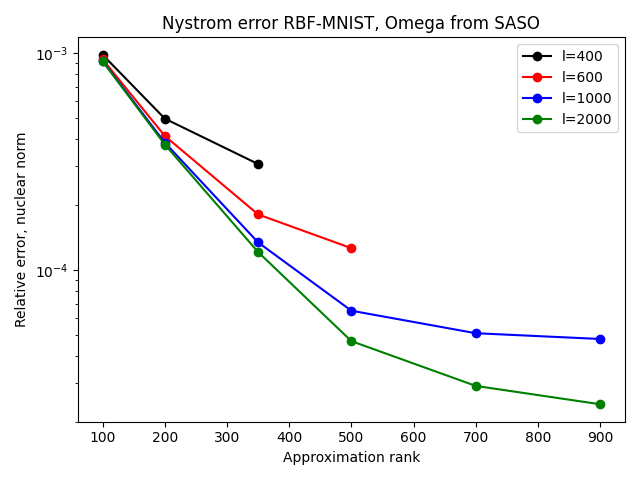
\includegraphics[width=\textwidth]{plots/relerror/relerror_RBF-MNIST_SASO.png}
    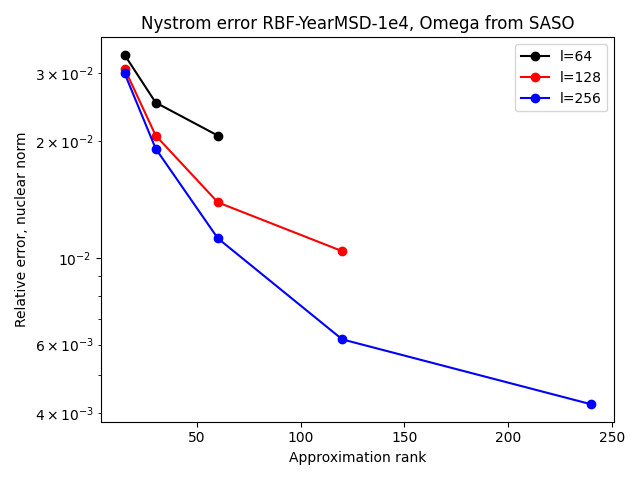
\includegraphics[width=\textwidth]{plots/relerror/relerror_RBF-YearMSD-1e4_SASO.png}
    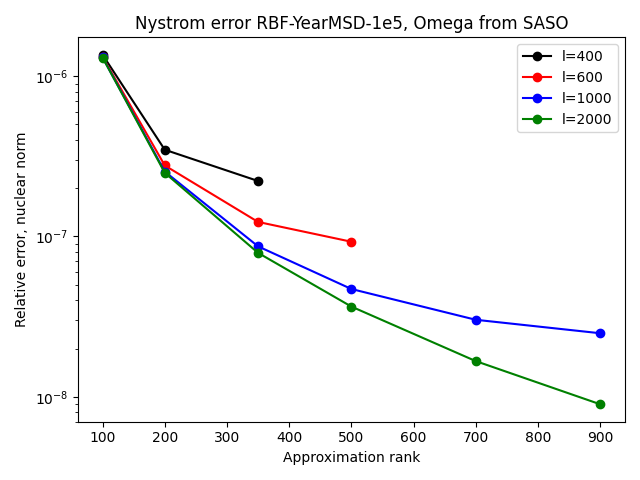
\includegraphics[width=\textwidth]{plots/relerror/relerror_RBF-YearMSD-1e5_SASO.png}
    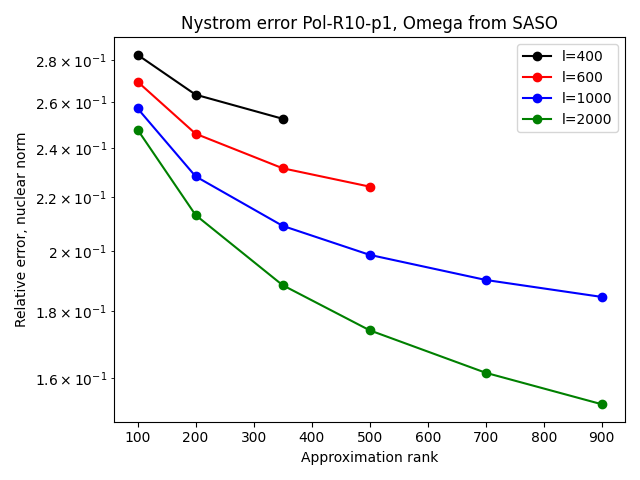
\includegraphics[width=\textwidth]{plots/relerror/relerror_Pol-R10-p1_SASO.png}
    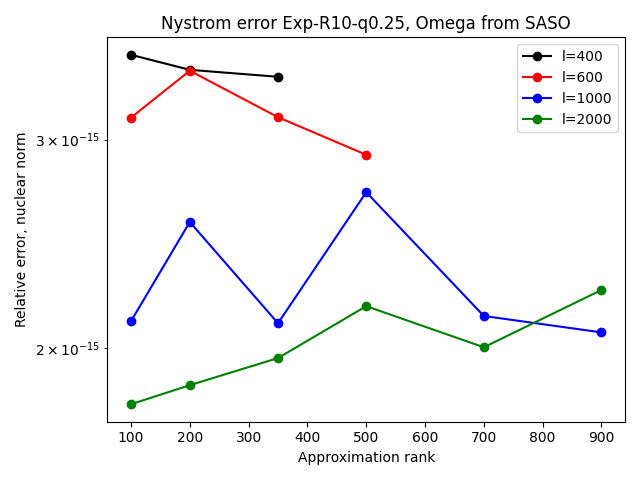
\includegraphics[width=\textwidth]{plots/relerror/relerror_Exp-R10-q0.25_SASO.png}
    \caption{$\Omega$ created using SASO}
\end{subfigure}\hfill
\caption{Relative error of the Nyström algorithm.}
\label{fig:RelError}
\end{figure}

\section{Runtime} \label{sec:performance}

We evaluated the runtime of the randomized Nyström algorithm on the same parameters as in section \ref{sec:num_stability}. The runtime was measured as the time to do the steps described in sections \ref{sec:rand_nystrom_alg} and \ref{sec:parallel_nystrom}, and thus does not include the time to generate the positive semi-definite matrix $A$ from the data $X$. To quantify the variation in runtimes, all tests were run 3 times to show the mean and the standard deviation of the runtimes at the different parameters. For the performance evaluation, we executed all algorithms on a single machine with an Intel Core i5 6500 ($4 \times 3.6$ GHz, $6$MB L3 cache) processor and 16 GB of DDR4-RAM powered by Fedora 38 (64-Bit, Linux Kernel $6.5.6$). Furthermore, the algorithms have been implemented in Python $3.11.5$ using NumPy $1.26.0$. The parallelization has been done via the Python implementation \textit{mpi4py} $3.1.4$ of the well-known Message Passing Interface (MPI) (OpenMPI 4.1.4).\newline


\subsection{Parallel runtime}
The parallel runtime, with the sketching matrices created using BSRHT and SASO, are shown in figure \ref{fig:Runtime}. We find that the exponential decay dataset is significantly slower than the other datasets. This difference comes down to the difference between the algorithms used, ***and fits with the theory described in section?????***. Besides the difference found between the two algorithms, we found little variation in the runtime across datasets. \newline

When selecting between the sketching dimension and the approximation rank, we see a large difference in runtimes. When increasing the sketching dimension, and thus working with larger sketched matrices $B$ and $C$, it takes significantly longer to run the approximation. We consistently saw an increase of runtime of more than a factor 3 when doubling the sketching dimension from $1000$ to $2000$. We also found that the increase in runtime when increasing the sketch dimension was larger than any of our increases in the approximation rank. This makes sense when looking back at section \ref{sec:parallel_nystrom}, where an increase in sketching dimension is directly related to the size of the matrices, $C_i\in\mathbb{R}^{n/\sqrt{P}\times l}$ and $B_{i,j}\in\mathbb{R}^{l\times l}$, and thus how many numbers we have to use in the calculation of the parallel randomized Nyström. On the other hand, the difference in runtime across the approximation rank only affects the final step described in section \ref{sec:parallel_nystrom}, where the rank-k truncated SVD is found, and the $\llbracket A_{Nyst}\rrbracket_k$ is calculated.

% No Q vs Q version. Describe our choice
% Runtime plots - describe what we see/have found

\begin{figure}
\centering
\hfill\begin{subfigure}[t]{\dimexpr0.4\textwidth+20pt\relax}
    \makebox[20pt]{\raisebox{65pt}{\rotatebox[origin=c]{90}{MNIST}}}%
    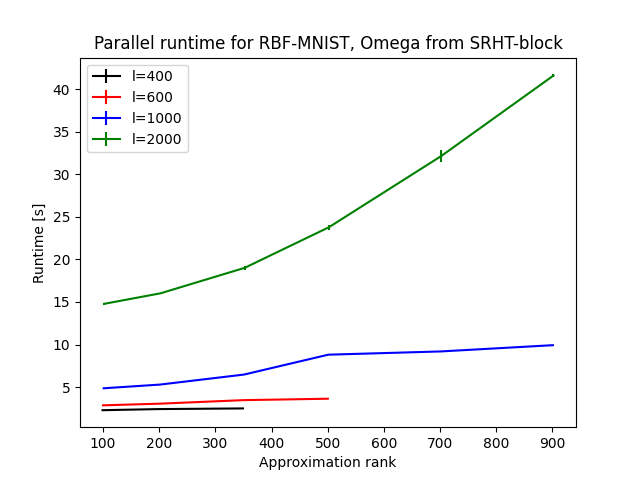
\includegraphics[width=\dimexpr\linewidth-20pt\relax]{plots/runtime_new/runtime_par_RBF-MNIST_SRHT-block.png}
    \makebox[20pt]{\raisebox{65pt}{\rotatebox[origin=c]{90}{YearMSD, $\sigma=10^4$}}}%
    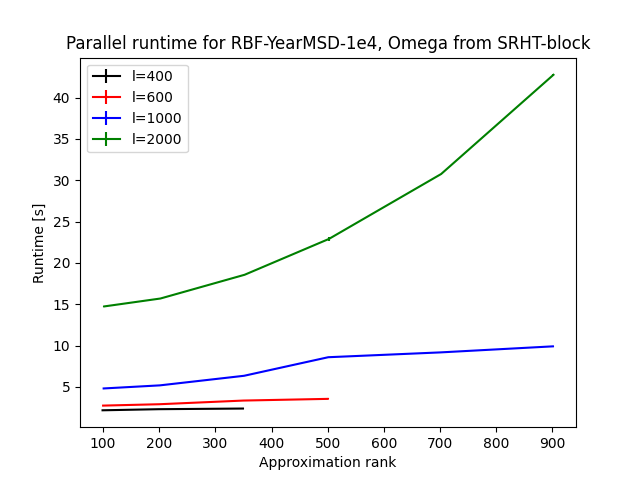
\includegraphics[width=\dimexpr\linewidth-20pt\relax]{plots/runtime_new/runtime_par_RBF-YearMSD-1e4_SRHT-block.png}
    \makebox[20pt]{\raisebox{65pt}{\rotatebox[origin=c]{90}{YearMSD, $\sigma=10^5$}}}%
    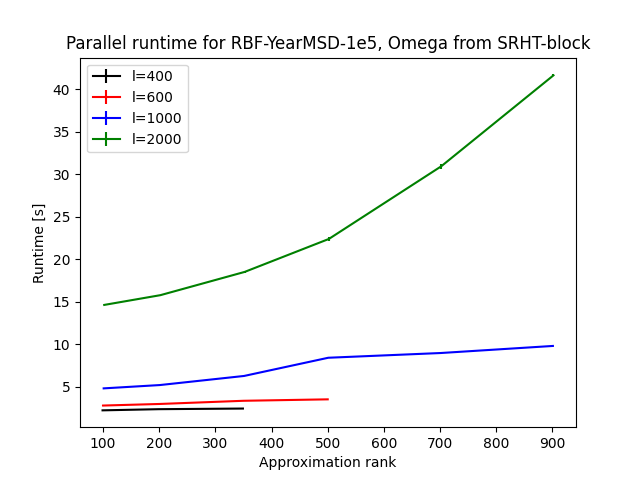
\includegraphics[width=\dimexpr\linewidth-20pt\relax]{plots/runtime_new/runtime_par_RBF-YearMSD-1e5_SRHT-block.png}
    \makebox[20pt]{\raisebox{65pt}{\rotatebox[origin=c]{90}{Polynomial decay}}}%
    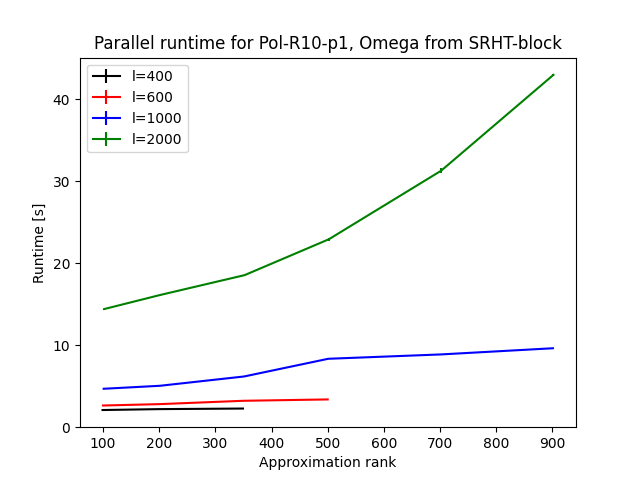
\includegraphics[width=\dimexpr\linewidth-20pt\relax]{plots/runtime_new/runtime_par_Pol-R10-p1_SRHT-block.png}
    \makebox[20pt]{\raisebox{65pt}{\rotatebox[origin=c]{90}{Exponential decay}}}%
    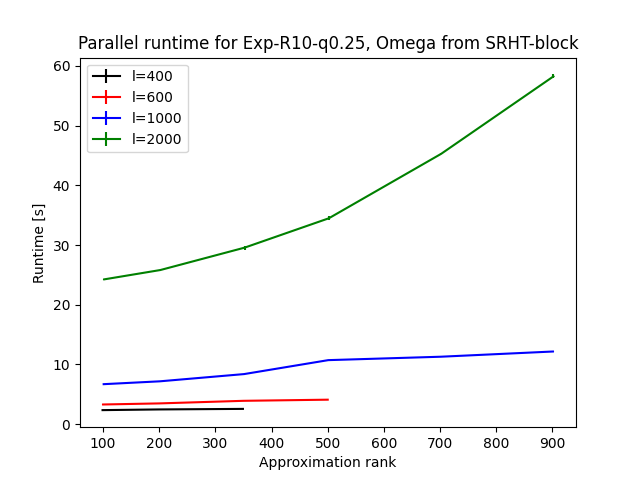
\includegraphics[width=\dimexpr\linewidth-20pt\relax]{plots/runtime_new/runtime_par_Exp-R10-q0.25_SRHT-block.png}
    \caption{$\Omega$ created using BSRHT}
\end{subfigure}\hfill
\begin{subfigure}[t]{0.4\textwidth}
    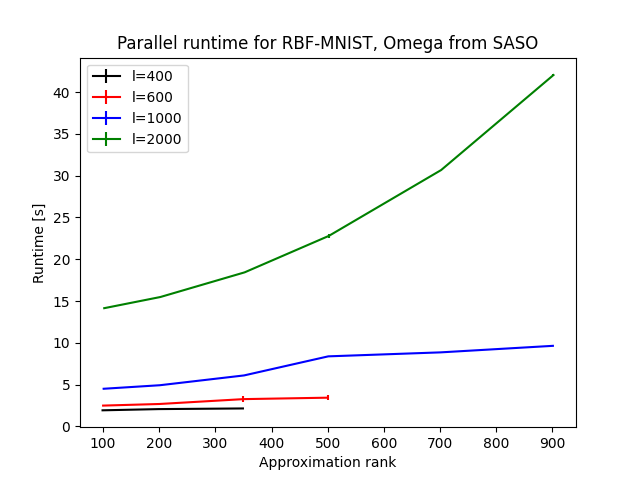
\includegraphics[width=\textwidth]{plots/runtime_new/runtime_par_RBF-MNIST_SASO.png}
    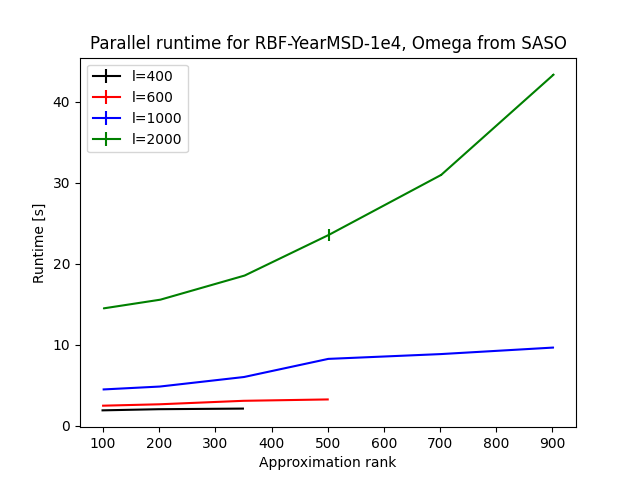
\includegraphics[width=\textwidth]{plots/runtime_new/runtime_par_RBF-YearMSD-1e4_SASO.png}
    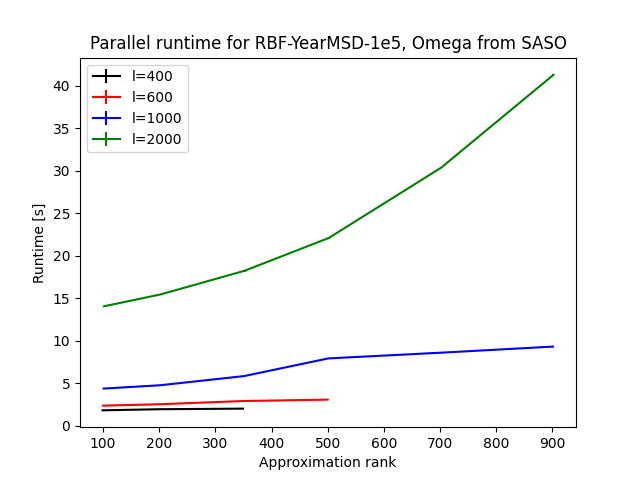
\includegraphics[width=\textwidth]{plots/runtime_new/runtime_par_RBF-YearMSD-1e5_SASO.png}
    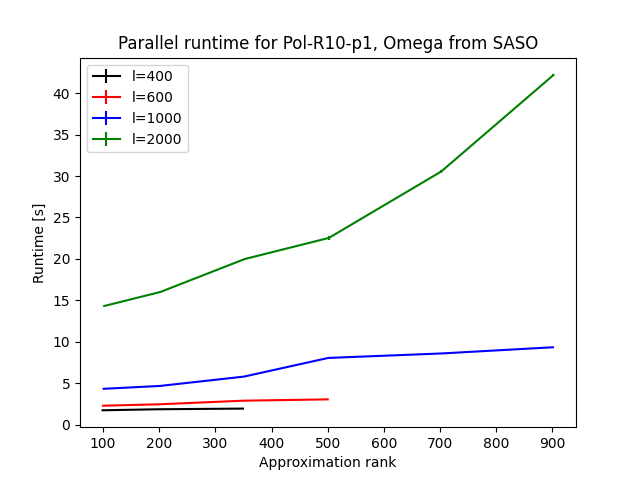
\includegraphics[width=\textwidth]{plots/runtime_new/runtime_par_Pol-R10-p1_SASO.png}
    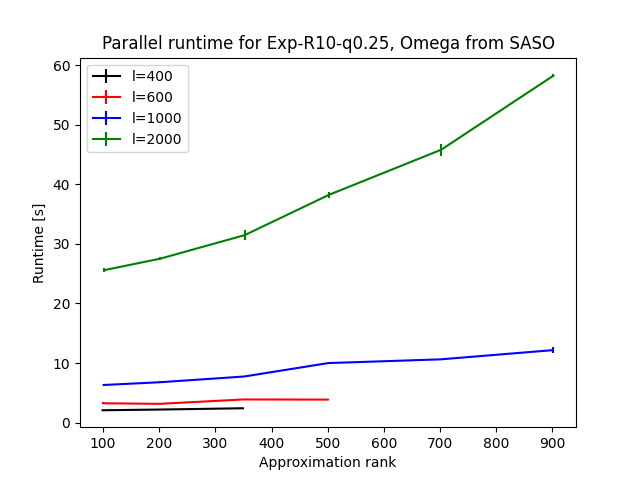
\includegraphics[width=\textwidth]{plots/runtime_new/runtime_par_Exp-R10-q0.25_SASO.png}
    \caption{$\Omega$ created using SASO}
\end{subfigure}\hfill
\caption{Runtime of the parallel Nyström algorithm.}
\label{fig:Runtime}
\end{figure}

\subsection{Sequential runtime}
***Missing sequential plots for SASO***

The sequential runtime, with the sketching matrices created using SRHT and SASO, are shown in figure \ref{fig:SequentialRuntime}. We find very similar internal comparisons between the different datasets. Since the exponential dataset is run using ***name of svd nystrom algorithm*** this has a much higher runtime than the other datasets, and increasing the approximation rank or the sketching dimension both increase the runtime. 

Comparing against the parallel runtime, we find that going from the parallel algorithm (with $4$ processors) to the sequential algorithm, the runtime increases by 30-50\%. This is a significant improvement, especially when the runtime is upwards of $60+$ seconds for some parameter settings with the sequential algorithm. However, as we have increased the number of processors by a factor of $4$, we do find an overhead when having to distribute and gather the workload across the different processors. ***What part of the algorithm took a whole, and was thus to blame for no further speedups???***

% Discuss if you observe any advantage in using a faster sketching operator with respect to the sketch dimension l that you might need in order to obtain an accurate low rank approximation.
Comparing the two different sketching matrices, we find that... ***missing sequential SASO runtimes***

\begin{figure}
\centering
\hfill\begin{subfigure}[t]{\dimexpr0.35\textwidth+20pt\relax}
    \makebox[20pt]{\raisebox{65pt}{\rotatebox[origin=c]{90}{MNIST}}}%
    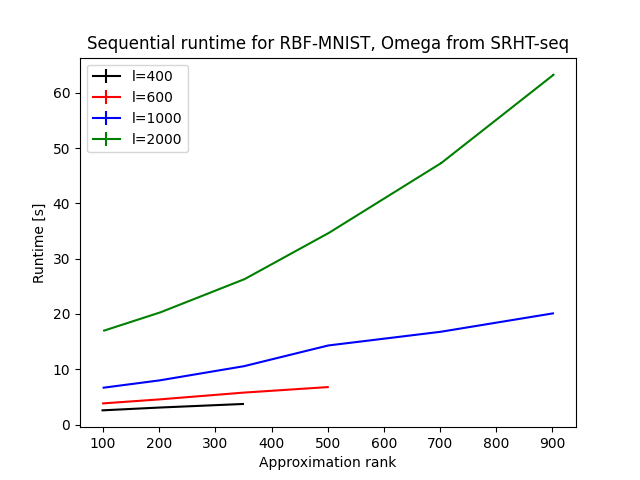
\includegraphics[width=\dimexpr\linewidth-20pt\relax]{plots/runtime_new/runtime_RBF-MNIST_SRHT-seq.png}
    \makebox[20pt]{\raisebox{65pt}{\rotatebox[origin=c]{90}{YearMSD, $\sigma=10^4$}}}%
    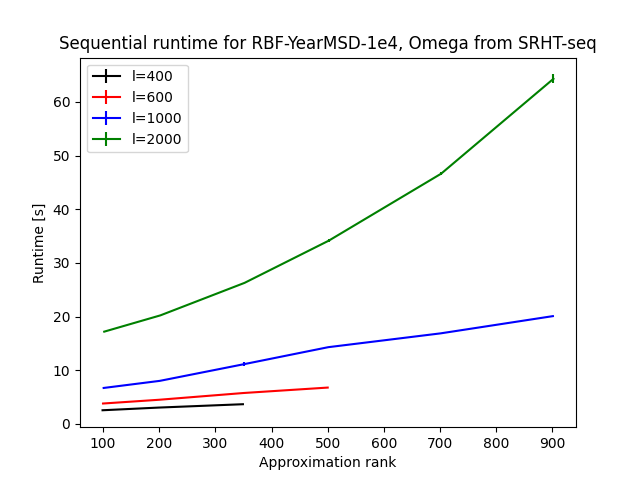
\includegraphics[width=\dimexpr\linewidth-20pt\relax]{plots/runtime_new/runtime_RBF-YearMSD-1e4_SRHT-seq.png}
    \makebox[20pt]{\raisebox{65pt}{\rotatebox[origin=c]{90}{YearMSD, $\sigma=10^5$}}}%
    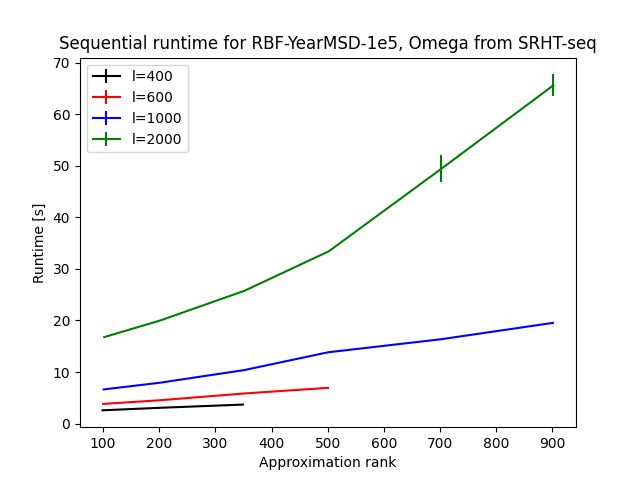
\includegraphics[width=\dimexpr\linewidth-20pt\relax]{plots/runtime_new/runtime_RBF-YearMSD-1e5_SRHT-seq.png}
    \makebox[20pt]{\raisebox{65pt}{\rotatebox[origin=c]{90}{Polynomial decay}}}%
    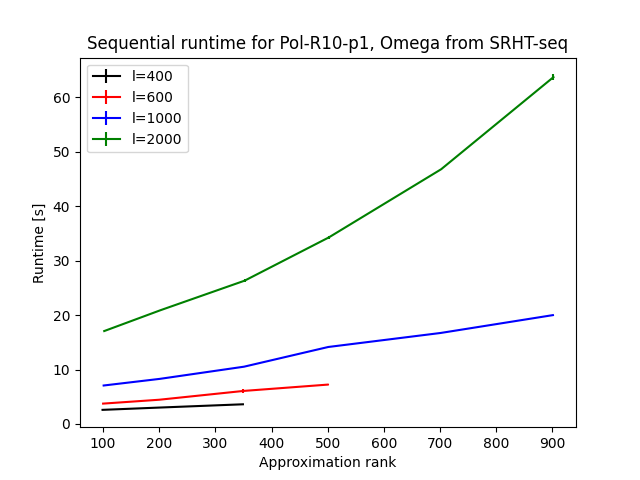
\includegraphics[width=\dimexpr\linewidth-20pt\relax]{plots/runtime_new/runtime_Pol-R10-p1_SRHT-seq.png}
    \makebox[20pt]{\raisebox{65pt}{\rotatebox[origin=c]{90}{Exponential decay}}}%
    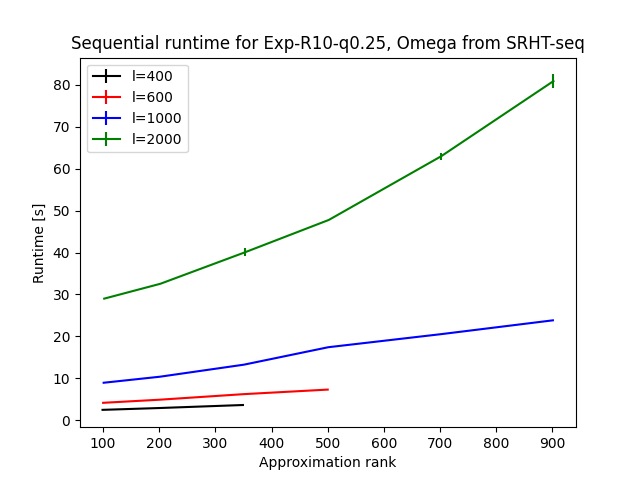
\includegraphics[width=\dimexpr\linewidth-20pt\relax]{plots/runtime_new/runtime_Exp-R10-q0.25_SRHT-seq.png}
    \caption{$\Omega$ created using SRHT}
\end{subfigure}\hfill
\begin{subfigure}[t]{0.35\textwidth}
    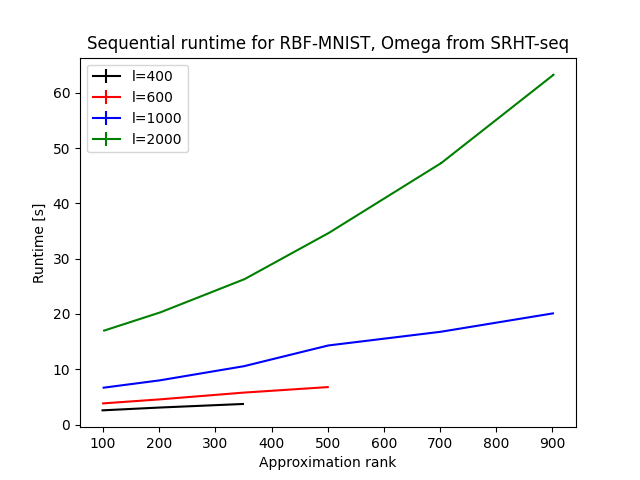
\includegraphics[width=\textwidth]{plots/runtime_new/runtime_RBF-MNIST_SRHT-seq.png}
    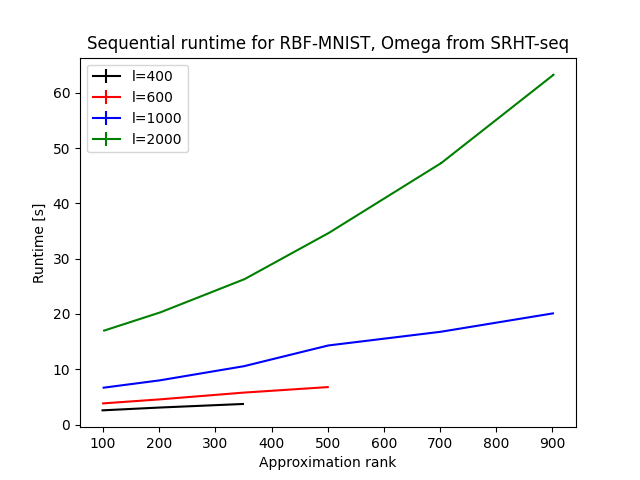
\includegraphics[width=\textwidth]{plots/runtime_new/runtime_RBF-MNIST_SRHT-seq.png}
    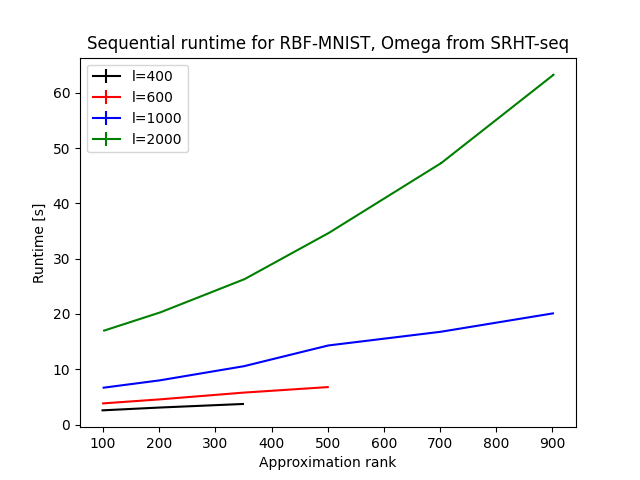
\includegraphics[width=\textwidth]{plots/runtime_new/runtime_RBF-MNIST_SRHT-seq.png}
    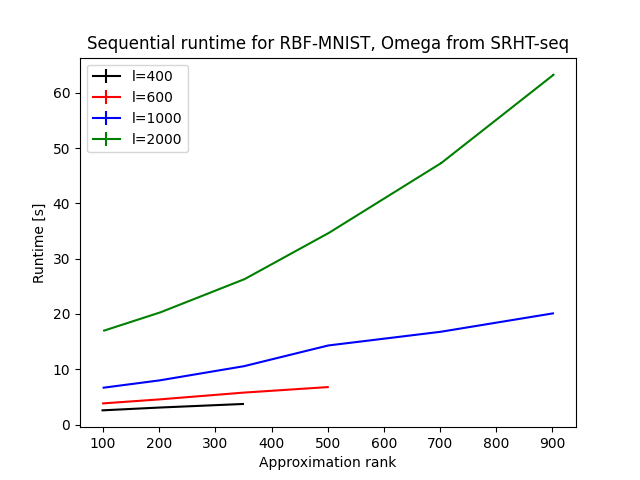
\includegraphics[width=\textwidth]{plots/runtime_new/runtime_RBF-MNIST_SRHT-seq.png}
    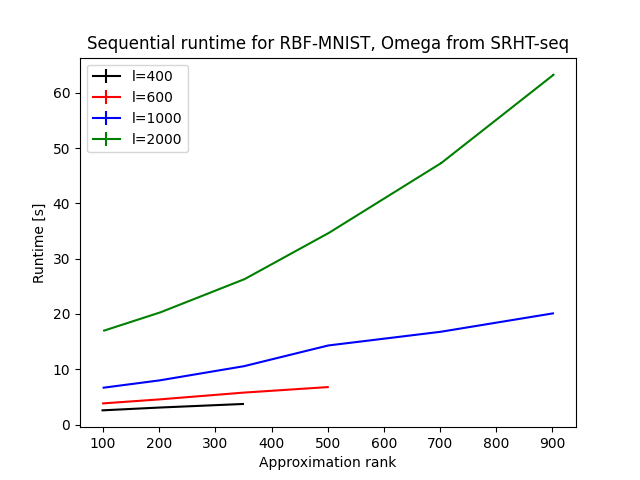
\includegraphics[width=\textwidth]{plots/runtime_new/runtime_RBF-MNIST_SRHT-seq.png}
    \caption{$\Omega$ created using SASO (SHOULD BE CHANGED TO RUNTIME OF SEQUENTIAL USING SASO!)}
\end{subfigure}\hfill
\caption{Runtime of the sequential version of the randomized Nyström algorithm.}
\label{fig:SequentialRuntime}
\end{figure}

\section{Approximation of leading Singular Values}

In this section, we address the question of whether the leading $k$ singular values of $A$ can be approximated using $[\![A_{Nystr}]\!]_k$. In particular, we compare the largest $k$ singular values of $A$ and $[\![A_{Nystr}]\!]_k$ (ordered in non-increasingly) and measure their difference in terms of the ratio
\begin{align}
    \label{eq:singularValueError}
    \text{error}_{\sigma_i} := \frac{\sigma_i([\![A_{Nystr}]\!]_k)}{\sigma_i(A)}
    \quad \forall i \in [k].
\end{align}

Figure \ref{} shows the results obtained for our four test matrices/datasets (MNIST, YearPredictionMSD, Polynomial Decay, Exponential Decay). The plots display the ratio (\ref{eq:singularValueError}) computed by SVD for the approximation rank $k=400$ and different sketching dimensions $l \in \{400, 600, 1000, 2000\}$.


% Create a plot where we find the true first k singular values, and the k singular values of the Nyström approx. We can then subtract them to get k different error values, whereby we can easily see the minimum and maximum error (and how it evolves throughout k) of the approximation to the true. This can be done for all the different datasets, and for a single choice of l and k.

\section{Conclusion}

\clearpage{}
% Moved bibliography above appendix
\printbibliography{} % print bibliography
\clearpage
\begin{appendices}
\section{Numerical Stability of Sequential Nyström}
\begin{figure}
\centering
\hfill\begin{subfigure}[t]{\dimexpr0.35\textwidth+20pt\relax}
    \makebox[20pt]{\raisebox{65pt}{\rotatebox[origin=c]{90}{MNIST}}}%
    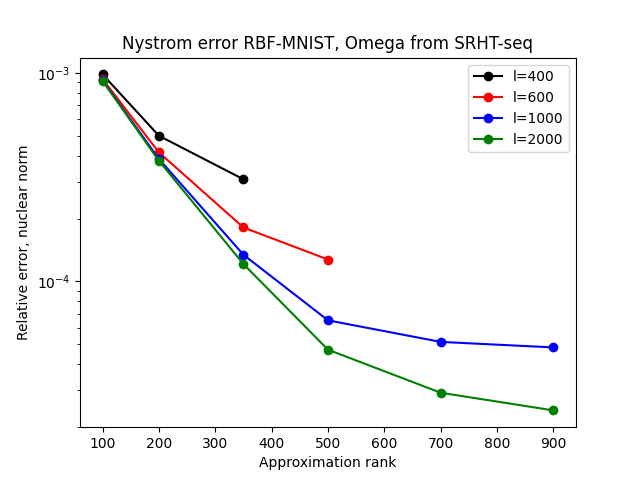
\includegraphics[width=\dimexpr\linewidth-20pt\relax]{plots/relerror/relerror_RBF-MNIST_SRHT-seq.png}
    \makebox[20pt]{\raisebox{65pt}{\rotatebox[origin=c]{90}{YearMSD, $\sigma=10^4$}}}%
    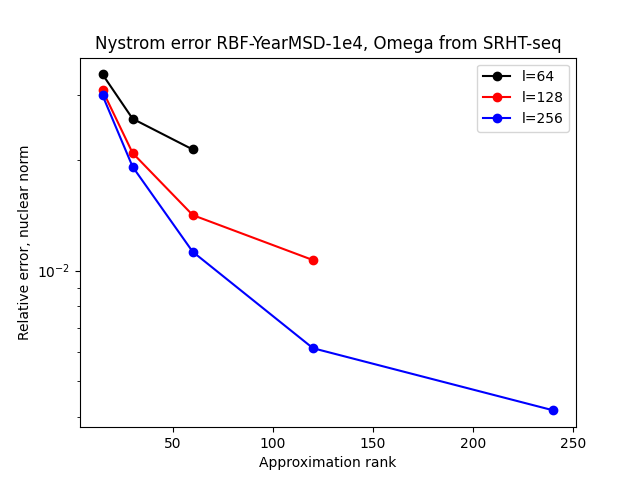
\includegraphics[width=\dimexpr\linewidth-20pt\relax]{plots/relerror/relerror_RBF-YearMSD-1e4_SRHT-seq.png}
    \makebox[20pt]{\raisebox{65pt}{\rotatebox[origin=c]{90}{YearMSD, $\sigma=10^5$}}}%
    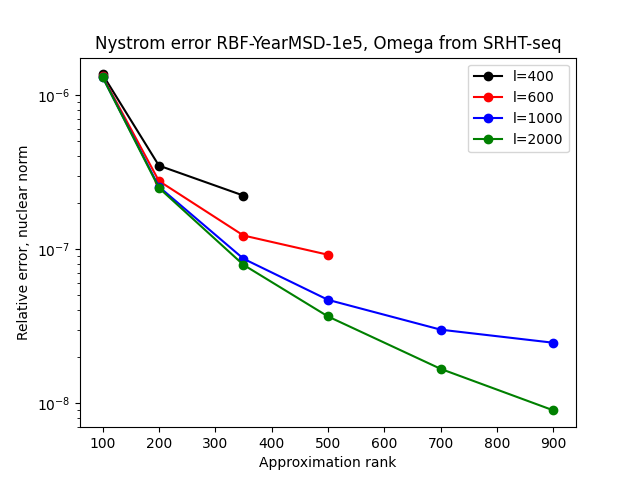
\includegraphics[width=\dimexpr\linewidth-20pt\relax]{plots/relerror/relerror_RBF-YearMSD-1e5_SRHT-seq.png}
    \makebox[20pt]{\raisebox{65pt}{\rotatebox[origin=c]{90}{Polynomial decay}}}%
    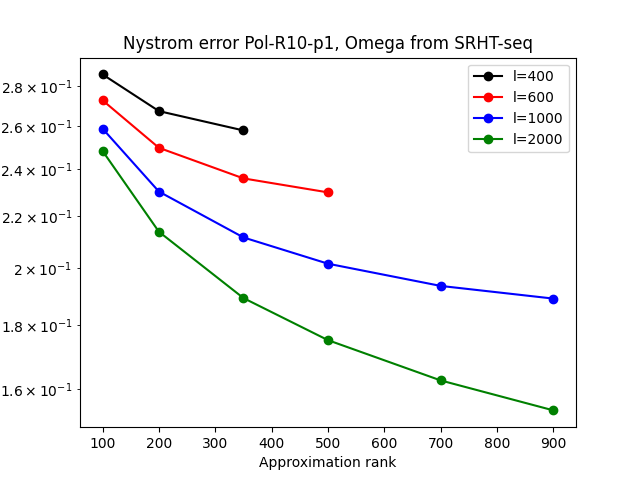
\includegraphics[width=\dimexpr\linewidth-20pt\relax]{plots/relerror/relerror_Pol-R10-p1_SRHT-seq.png}
    \makebox[20pt]{\raisebox{65pt}{\rotatebox[origin=c]{90}{Exponential decay}}}%
    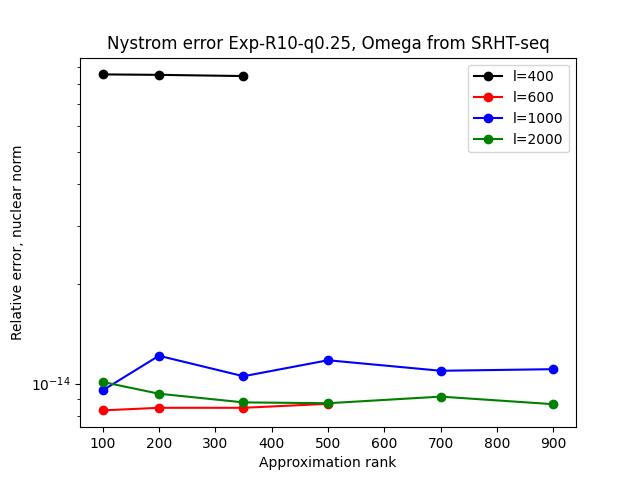
\includegraphics[width=\dimexpr\linewidth-20pt\relax]{plots/relerror/relerror_Exp-R10-q0.25_SRHT-seq.png}
    \caption{$\Omega$ created using BSRHT}
\end{subfigure}\hfill
\begin{subfigure}[t]{0.35\textwidth}
    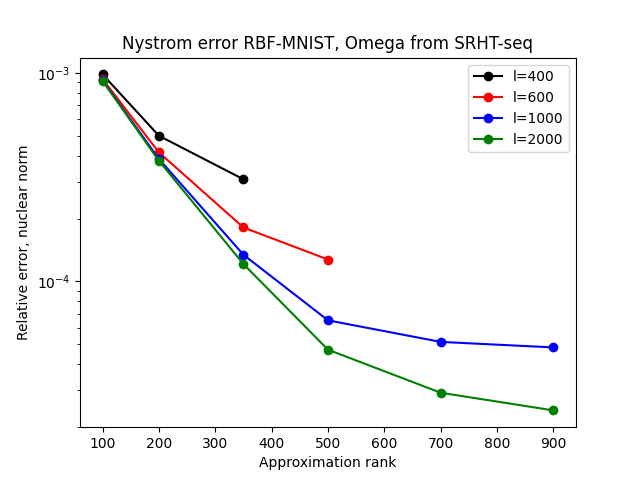
\includegraphics[width=\textwidth]{plots/relerror/relerror_RBF-MNIST_SRHT-seq.png}
    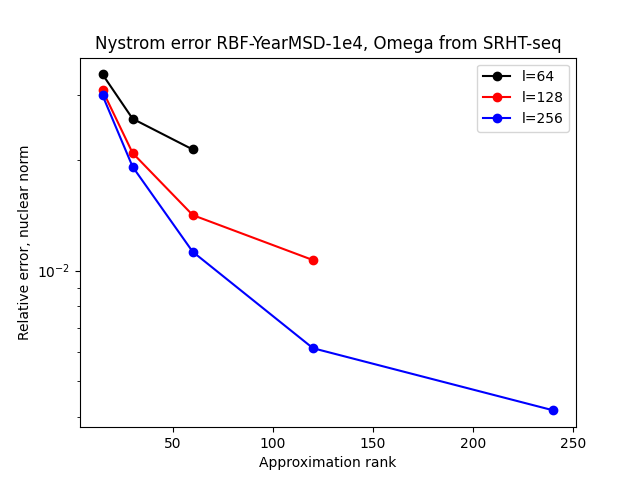
\includegraphics[width=\textwidth]{plots/relerror/relerror_RBF-YearMSD-1e4_SRHT-seq.png}
    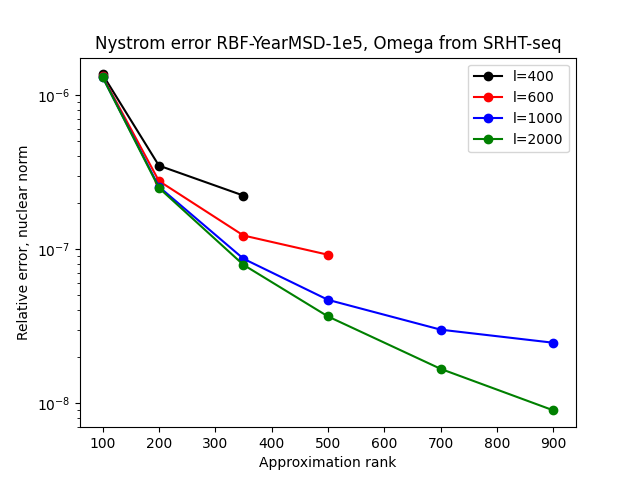
\includegraphics[width=\textwidth]{plots/relerror/relerror_RBF-YearMSD-1e5_SRHT-seq.png}
    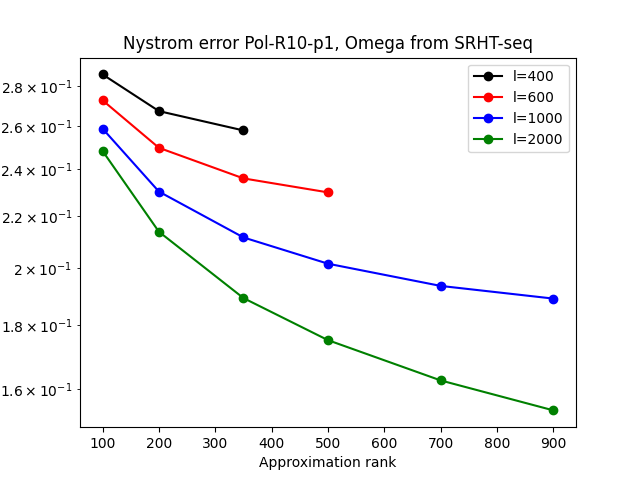
\includegraphics[width=\textwidth]{plots/relerror/relerror_Pol-R10-p1_SRHT-seq.png}
    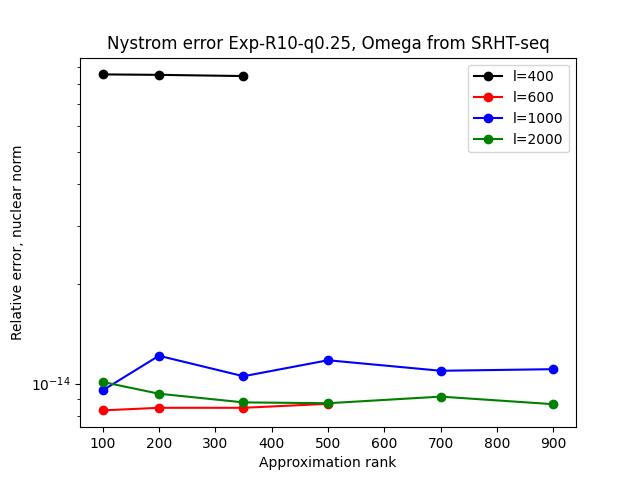
\includegraphics[width=\textwidth]{plots/relerror/relerror_Exp-R10-q0.25_SRHT-seq.png}
    \caption{$\Omega$ created using SASO (SHOULD BE CHANGED TO NUMERICAL PERFORMANCE OF SEQUENTIAL ALGORITHMS!)}
\end{subfigure}\hfill
\caption{Relative error of the sequential version of the randomized Nyström algorithm with different sketching matrices. Created for comparison with figure \ref{fig:RelError} ***but found to have similar results????***.}
\label{fig:SequentialRelError}
\end{figure}
\end{appendices}


\end{document}
